\subsection{Backpropagation for a simple network}

\subsubsection{Formeln für Forwardfeed}

Zuerst werden die Eingänge entsprechend der W(1)-Matrix gewichtet und aufsummiert.
\begin{equation}
\vect{a}^{(1)} = [\vect{x},1] * \vect{W}^{(1)}
\end{equation}

Die Summe der gewichteten Eingänge wird anschließend durch die Aktivierungsfunktion $\sigma(x)$ geschickt.

\begin{equation}
\vect{z} = \sigma(\vect{a}^{(1)})
\end{equation}

Anschließend wird werden die Ausgänge der Neuronen (z) mit der W(2)-Matrix gewichichtet und aufsummiert:

\begin{equation}
 \vect{a}^{(2)} = [z,1] * \vect{W}^{(2)}
\end{equation}

Die Summe der gewichteten Neuronenausgänge im Hidden Layer wird anschließend wieder durch die Aktivierungsfunktion $\sigma(x)$ geschickt.
\begin{equation}
 output = \sigma(\vect{a}^{(2)})
\end{equation}




\begin{figure}[hp!]
\begin{center}
 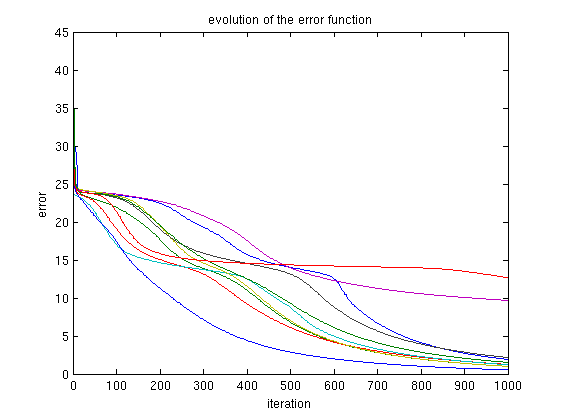
\includegraphics[width=0.99\textwidth]{./figures/1/error}
 \caption{Evolution of the error over the iterations with different startweight-vectors}
\label{fig:backprop_error}
\end{center}
\end{figure}



\begin{figure}[hp!]
\begin{center}
 \begin{minipage}{0.48\textwidth}
 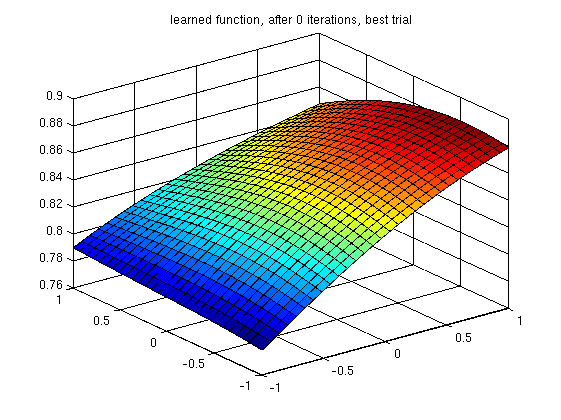
\includegraphics[width=0.99\textwidth]{./figures/1/learned_best_0}
 \end{minipage}
 \begin{minipage}{0.48\textwidth}
 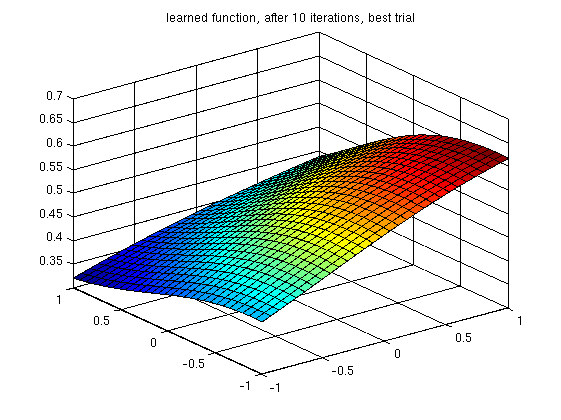
\includegraphics[width=0.99\textwidth]{./figures/1/learned_best_10}
 \end{minipage}
 \begin{minipage}{0.48\textwidth}
 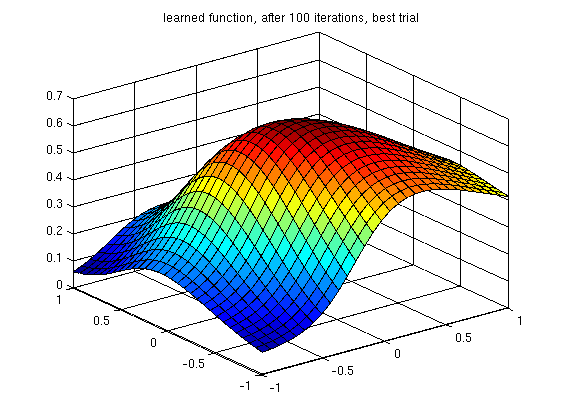
\includegraphics[width=0.99\textwidth]{./figures/1/learned_best_100}
 \end{minipage}
 \begin{minipage}{0.48\textwidth}
 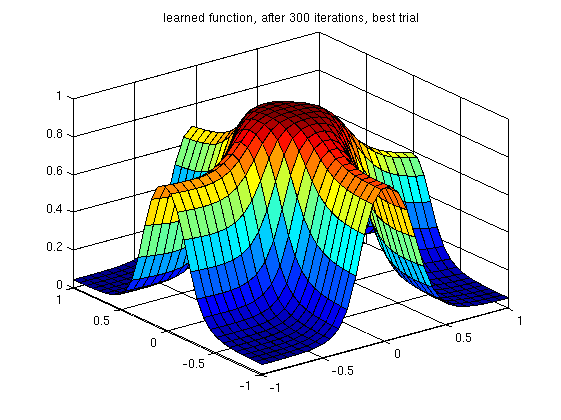
\includegraphics[width=0.99\textwidth]{./figures/1/learned_best_300}
 \end{minipage}
 \begin{minipage}{0.48\textwidth}
 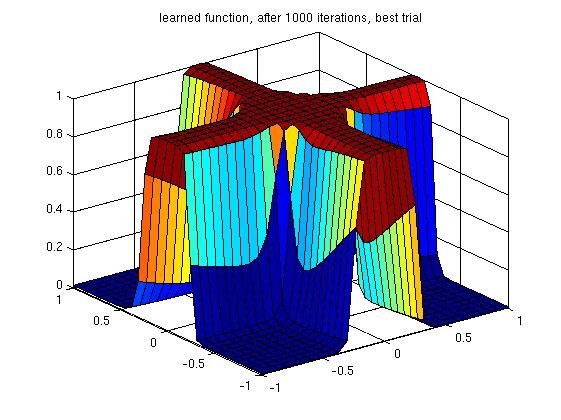
\includegraphics[width=0.99\textwidth]{./figures/1/learned_best_1000}
 \end{minipage}
 \caption{Learned Function after 0,10,100,300,1000 Iterations(Best Trial)}
\label{fig:learned_function_best}
\end{center}
\end{figure}


\begin{figure}[hp!]
\begin{center}
 \begin{minipage}{0.48\textwidth}
 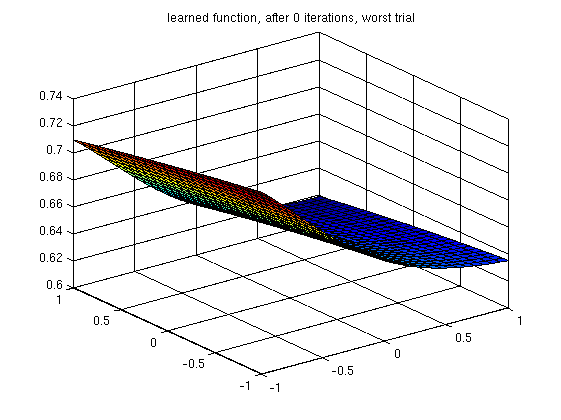
\includegraphics[width=0.99\textwidth]{./figures/1/learned_worst_0}
 \end{minipage}
 \begin{minipage}{0.48\textwidth}
 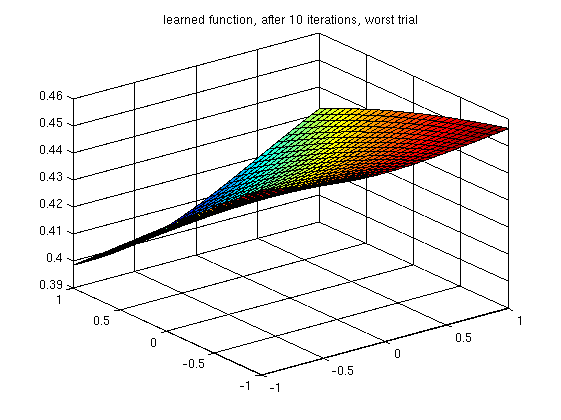
\includegraphics[width=0.99\textwidth]{./figures/1/learned_worst_10}
 \end{minipage}
 \begin{minipage}{0.48\textwidth}
 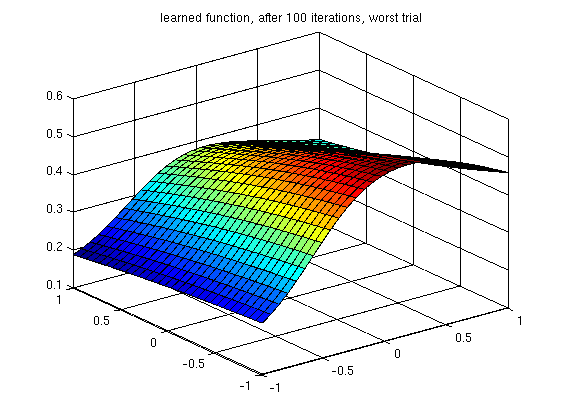
\includegraphics[width=0.99\textwidth]{./figures/1/learned_worst_100}
 \end{minipage}
 \begin{minipage}{0.48\textwidth}
 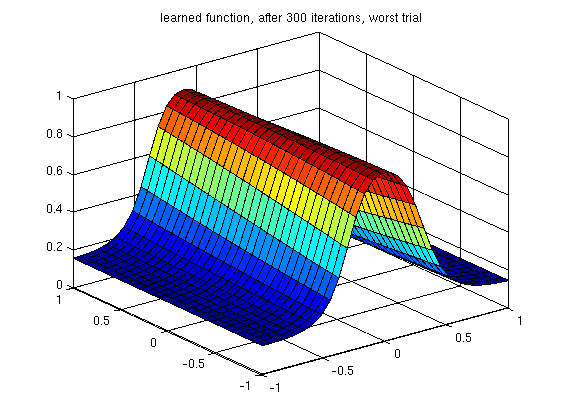
\includegraphics[width=0.99\textwidth]{./figures/1/learned_worst_300}
 \end{minipage}
 \begin{minipage}{0.48\textwidth}
 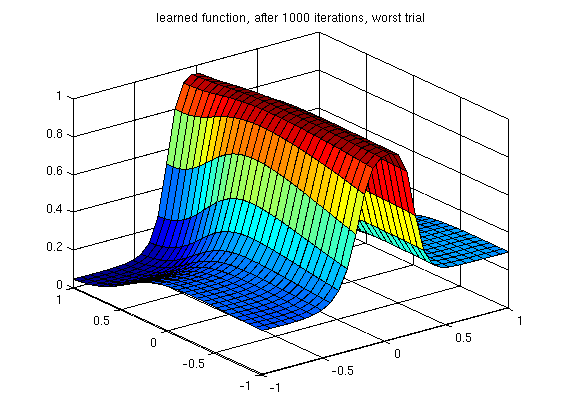
\includegraphics[width=0.99\textwidth]{./figures/1/learned_worst_1000}
 \end{minipage}
 \caption{Learned Function after 0,10,100,300,1000 Iterations(Worst Trial)}
\label{fig:learned_function_worst}
\end{center}
\end{figure}

